\documentclass[border=9pt]{standalone}
\usepackage{amsmath,amssymb}
\usepackage{tikz-cd}
\usetikzlibrary{calc}
\definecolor{chord}{RGB}{37,99,163}
\definecolor{returnline}{RGB}{195,85,35}
\definecolor{curve}{RGB}{50,57,66}
% An exact projective cubic: C: yz^2=x^3.
% In z=1, p(t)=(t,t^3). Its flex P_0=p(0) is regular.
% Three distinct points p(a),p(b),p(c) are collinear iff a+b+c=0.
% Thus choose P_1=p(.35), P_2=p(.70), P_3=p(-1.65).
% The cusp [0:1:0] is outside this affine chart.
% Saveboxes avoid nesting an active tikzpicture inside tikzcd.
\newsavebox{\firstleft}
\newsavebox{\firstright}
\newsavebox{\secondleft}
\newsavebox{\secondright}
\tikzset{
  point/.style={circle,fill=curve,inner sep=1.65pt},
  result/.style={circle,fill=returnline,inner sep=2pt},
  lab/.style={font=\small,fill=white,inner sep=1.5pt,text=black},
  ch/.style={chord,line width=.9pt},
  ret/.style={returnline,dashed,line width=.9pt}
}
% All coordinates in each panel use x=2.25cm, y=.48cm.
\newcommand{\basecurve}{
  \path[use as bounding box] (-2,-6.7) rectangle (2,6.7);
  \begin{scope}
    \clip (-1.88,-6.2) rectangle (1.88,6.2);
    \draw[curve,line width=1.1pt,samples=180,domain=-1.8:1.8]
      plot (\x,{\x*\x*\x});
  \end{scope}
  \node[lab,text=curve] at (1.63,5.75) {$C$};
}
% Chord through p(a),p(b): y=(a^2+ab+b^2)x-ab(a+b).
\newcommand{\chordline}[2]{
 \begin{scope}
  \clip (-1.88,-6.2) rectangle (1.88,6.2);
  \draw[ch,domain=-2:2] plot
   (\x,{((#1)^2+(#1)*(#2)+(#2)^2)*\x-(#1)*(#2)*((#1)+(#2))});
 \end{scope}
}
% Line through P_0 and p(r): y=r^2*x.
\newcommand{\returnthrough}[1]{
 \begin{scope}
  \clip (-1.88,-6.2) rectangle (1.88,6.2);
  \draw[ret] (-2,{-2*(#1)^2}) -- (2,{2*(#1)^2});
 \end{scope}
}
\newcommand{\pt}[4]{
 \node[#4] at (#1,{(#1)^3}) {};
 \node[lab,#3] at (#1,{(#1)^3}) {$#2$};
}
\begin{document}
\sbox{\firstleft}{
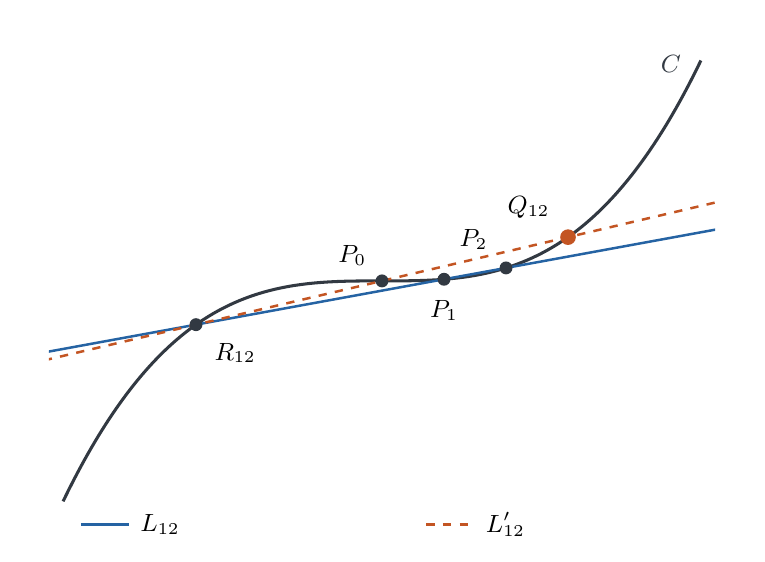
\begin{tikzpicture}[x=2.25cm,y=.48cm]
 \basecurve
 \chordline{.35}{.70}
 \returnthrough{-1.05}
 \pt{0}{P_0}{above left=4pt}{point}
 \pt{.35}{P_1}{below=6pt}{point}
 \pt{.70}{P_2}{above left=5pt}{point}
 \pt{-1.05}{R_{12}}{below right=5pt}{point}
 \pt{1.05}{Q_{12}}{above left=5pt}{result}
 \draw[ch] (-1.70,-6.45)--(-1.43,-6.45);
 \node[lab,anchor=west] at (-1.39,-6.45) {$L_{12}$};
 \draw[ret] (.25,-6.45)--(.52,-6.45);
 \node[lab,anchor=west] at (.56,-6.45) {$L'_{12}$};
\end{tikzpicture}}
\sbox{\firstright}{
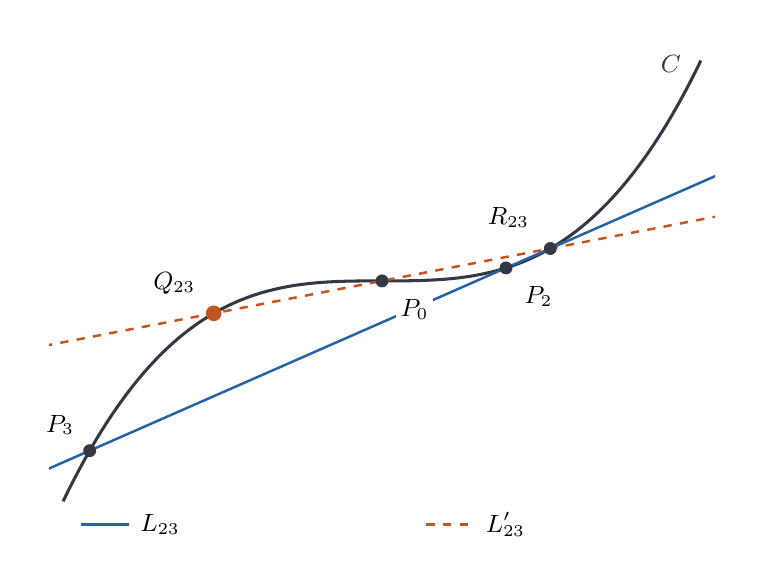
\begin{tikzpicture}[x=2.25cm,y=.48cm]
 \basecurve
 \chordline{.70}{-1.65}
 \returnthrough{.95}
 \pt{0}{P_0}{below right=5pt}{point}
 \pt{.70}{P_2}{below right=5pt}{point}
 \pt{-1.65}{P_3}{above left=4pt}{point}
 \pt{.95}{R_{23}}{above left=6pt}{point}
 \pt{-.95}{Q_{23}}{above left=5pt}{result}
 \draw[ch] (-1.70,-6.45)--(-1.43,-6.45);
 \node[lab,anchor=west] at (-1.39,-6.45) {$L_{23}$};
 \draw[ret] (.25,-6.45)--(.52,-6.45);
 \node[lab,anchor=west] at (.56,-6.45) {$L'_{23}$};
\end{tikzpicture}}
\sbox{\secondleft}{
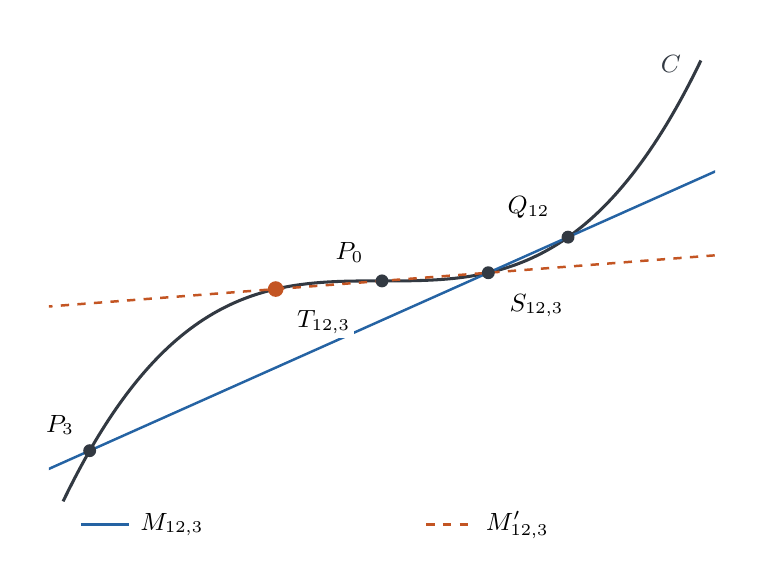
\begin{tikzpicture}[x=2.25cm,y=.48cm]
 \basecurve
 \chordline{1.05}{-1.65}
 \returnthrough{.60}
 \pt{0}{P_0}{above left=5pt}{point}
 \pt{1.05}{Q_{12}}{above left=5pt}{point}
 \pt{-1.65}{P_3}{above left=4pt}{point}
 \pt{.60}{S_{12,3}}{below right=6pt}{point}
 \pt{-.60}{T_{12,3}}{below right=6pt}{result}
 \draw[ch] (-1.70,-6.45)--(-1.43,-6.45);
 \node[lab,anchor=west] at (-1.39,-6.45) {$M_{12,3}$};
 \draw[ret] (.25,-6.45)--(.52,-6.45);
 \node[lab,anchor=west] at (.56,-6.45) {$M'_{12,3}$};
\end{tikzpicture}}
\sbox{\secondright}{
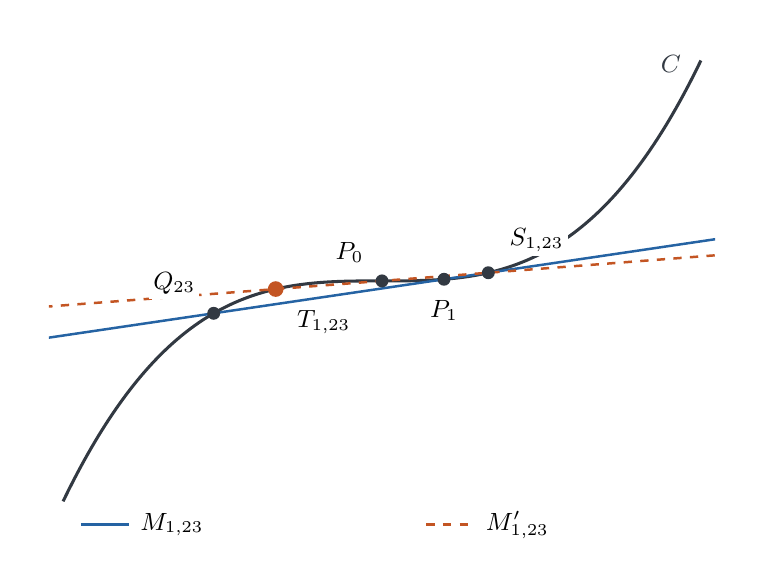
\begin{tikzpicture}[x=2.25cm,y=.48cm]
 \basecurve
 \chordline{.35}{-.95}
 \returnthrough{.60}
 \pt{0}{P_0}{above left=5pt}{point}
 \pt{.35}{P_1}{below=6pt}{point}
 \pt{-.95}{Q_{23}}{above left=5pt}{point}
 \pt{.60}{S_{1,23}}{above right=6pt}{point}
 \pt{-.60}{T_{1,23}}{below right=6pt}{result}
 \draw[ch] (-1.70,-6.45)--(-1.43,-6.45);
 \node[lab,anchor=west] at (-1.39,-6.45) {$M_{1,23}$};
 \draw[ret] (.25,-6.45)--(.52,-6.45);
 \node[lab,anchor=west] at (.56,-6.45) {$M'_{1,23}$};
\end{tikzpicture}}
\begin{minipage}{20cm}
\centering
{\small Left: $(P_1+P_2)+P_3$ \qquad\qquad Right: $P_1+(P_2+P_3)$}\\[9pt]
\begin{tikzcd}[column sep=1cm,row sep=1.3cm,
 cells={nodes={inner sep=0pt}},arrows={line width=.6pt}]
 {\usebox{\firstleft}}
 \arrow[d,"{\scriptstyle Q_{12}=P_1+P_2;\ \text{now add }P_3}"']
 &
 {\usebox{\firstright}}
 \arrow[d,"{\scriptstyle Q_{23}=P_2+P_3;\ \text{now add }P_1}"]
 \\
 {\usebox{\secondleft}} & {\usebox{\secondright}}
\end{tikzcd}
\\[8pt]
$\displaystyle T_{12,3}=(P_1+P_2)+P_3
       =P_1+(P_2+P_3)=T_{1,23}.$\\[9pt]
\small

\end{minipage}
\end{document}

